\documentclass[]{beamer}
% Class options include: notes, notesonly, handout, trans,
%                        hidesubsections, shadesubsections,
%                        inrow, blue, red, grey, brown

% Theme for beamer presentation.
\usepackage{beamerthemesplit} 
%\usepackage{times}
\usepackage{anysize}
\usepackage{fancyhdr}
\usepackage{graphicx}
\usepackage{pdfpages}
\usepackage[fleqn]{amsmath}
\usepackage{amssymb}
% Other themes include: beamerthemebars, beamerthemelined, 
%                       beamerthemetree, beamerthemetreebars  

\title{Jafar --- Intelligent Othello Agent}    % Enter your title between curly braces
\author{Joshua Nelson, Tim Cosgrove, Andrew Haigh}                 % Enter your name between curly braces
\institute{COMP3130 Research Project}      % Enter your institute name between curly braces
\date{\today}                    % Enter the date or \today between curly braces

\usetheme{PaloAlto}
\usecolortheme{crane}

\begin{document}

% Creates title page of slide show using above information
\begin{frame}
  \titlepage
\end{frame}
\note{} % Add notes to yourself that will be displayed when
        % typeset with the notes or notesonly class options

\section[Outline]{}

% Creates table of contents slide incorporating
% all \section and \subsection commands
\begin{frame}
  \tableofcontents
\end{frame}


\section{Problem Overview}

\begin{frame}
  \frametitle{Problem Overview}   % Insert frame title between curly braces
  \begin{columns}[c]
  \column{2in}  % slides are 3in high by 5in wide
  \begin{itemize}
  \item<1-> The Game --- 10x10 Modified Othello
  \item<2-> The Problem --- Intelligent AI player
  \item<3-> Solution basis
  \end{itemize}
  \column{2in}
  \framebox{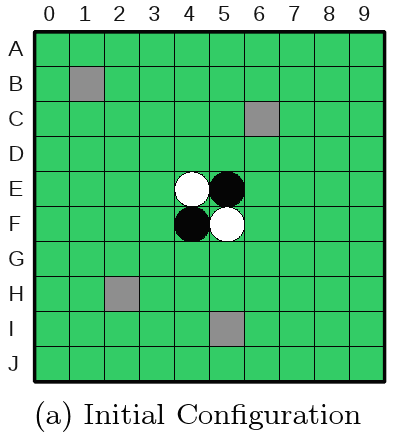
\includegraphics[height=5cm]{initconfig}}
  \end{columns}
\end{frame}

\end{document}
